% !TEX root = ./../../_Thesis.tex

% section's Name and Label
\subsection{Vertex Distance and Ray Transfer Matrix}
\label{subsec:ABCDMatrix}

\begin{figure}[!b]
	\centering

	\subfigure[]{
		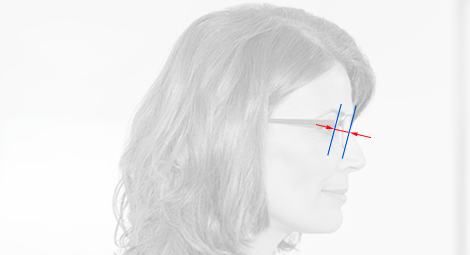
\includegraphics[width=0.40\linewidth]{__Images/04/Zeiss_BackVD.png}
		\label{fig:vertexdistance}
	}
	~
	\subfigure[]{
				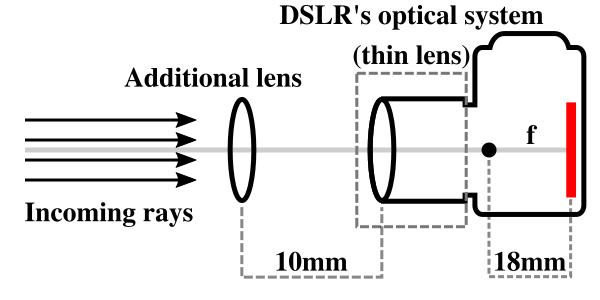
\includegraphics[width=0.55\linewidth]{__Images/04/RTM.png}
		\label{fig:rtm_scheme}
	}
	
	\caption[Vertex distance and our optical setup]{Vertex distance. (a) Typical eyeglasses vertex distance of 12mm. (b) Our camera setup with a distance of 10mm between DSLR's main lens and the additional one.}
	\label{fig:rtm}
\end{figure}

The optical power of a lens prescribed for correcting low-order aberrations varies according to the distance from the lens to the cornea, also known as {\it vertex distance} (Figure~\ref{fig:vertexdistance}). 
%While the vertex distance from the cornea to a contact lens is 0mm, its distance to an eyeglass is usually 12mm. 
To compensate for the spacing between camera's main lens and the additional ones (Figure~\ref{fig:rtm_scheme}), we use a {\it ray transfer matrix} (RTM) formulation 
%to describe the light path through the optical system 
\cite{Glytsis2014}.
%provides a step-by-step description of the process involved in computing a ray transfer matrix.
%This calculus, demonstrated step by step by \citet{Glytsis2014}, implicates in the determination of a new focal length and magnification value for the focal system consisting of two lens (\review{see Appendix XYZ}).
%Annex~\ref{chap:Annex1} discusses how to obtain the new focal length and magnification value for an optical system consisting of multiple lenses.
The RTM representing two thin lenses separated by a distance $d$ can be obtained multiplying three matrices:
%eq:W
 a thin lens matrix (that approximates the DSLR's optical system by a single thin lens), a distance $d$ propagation matrix, and a thin lens matrix representing our additional lenses:
%
\begin{equation}
	\centering
	\label{eq:RTM_tl}
	\begin{array} {lcl} \begin{bmatrix} A_{TL} & B_{TL}\\ C_{TL} & D_{TL} \end{bmatrix} 
	& = & \begin{bmatrix} 1 & 0\\ -\frac{1}{f_{camera}} & 1 \end{bmatrix}
	\begin{bmatrix} 1 & d\\ 0 & 1 \end{bmatrix}
	\begin{bmatrix} 1 & 0\\ -\frac{1}{f_{lens}} & 1 \end{bmatrix} \\ \\ 
	& = & \begin{bmatrix}
	1 - \dfrac{d}{f_{camera}} & d\\
	\left (  \dfrac{\dfrac{d}{f_{lens}}-1}{f_{camera}} - \dfrac{1}{f_{lens}}\right ) & 1 - \dfrac{d}{f_{lens}}
	\end{bmatrix}. 
	\end{array}
\end{equation}
%
Here $f_{camera}$ is the DLSR camera focal length (\ie, 18mm in our case), and $f_{lens}$ is the focal length of the (combined set of) additional lens(es).
The image captured by the resulting optical system is formed at a distance $x$ behind the DSLR camera's optical system. Assuming we want to capture the image of an infinitely far away object (\eg, at distance $s = 10^{20}$mm from the camera), the overall RTM can computed as:
%
\begin{equation}
	\centering
	\label{eq:RTM_final}
	\begin{bmatrix} A & B\\ C & D \end{bmatrix}
	=
	\begin{bmatrix} 1 & x\\ 0 & 1 \end{bmatrix}
	\begin{bmatrix} A_{TL} & B_{TL}\\ C_{TL} & D_{TL} \end{bmatrix}
	\begin{bmatrix} 1 & s\\ 0 & 1 \end{bmatrix}.
\end{equation}
%
Since a set of parallel rays (of an infinitely far away object) are focused by a lens to its focal point, one concludes that $x$ should indeed be the focal length $f_{cam+lens}$ of the compounded optical system comprised by the camera's main lens plus the additional one. 
%converge to the optical system's focal point, 
By letting $B = 0$, 
%\review{(justificar por que isso)}, 
one can solve for $x$, obtaining:
%To achieve optical system's new focal length, the ABCD matrix element $B$ must become zero. When $B = 0$, the value of $x$ gives the new focal length and the value of $A$ gives the overall magnification $m$ of the image (\ie, $m = A(x)$).
%
\begin{equation}
x = f_{cam+lens} = \dfrac{(d  + s) \times (f_{camera} \times f_{lens}) - (d \times f_{lens} \times s) }
{(d - f_{lens}) \times f_{camera} + (f_{camera} + f_{lens} - d )\times s}. 
\label{RTMx}
\end{equation}
%
%\begin{subequations}
 %\begin{align}
  %B = 0 \label{RTMb} \\
  %d + s\left (  x\left (\dfrac{ \dfrac{d}{f_{lens}}-1}{f_{camera}} - \dfrac{1}{f_{lens}}\right )-\dfrac{d}{f_{camera}}+1\right ) -x\left (\dfrac{d}{f_{lens}}-1\right ) = 0 \label{RTMb0} \\
  %x = \dfrac{d~f_{camera}~f_{lens} - d~f_{lens}~s+f_{camera}~f_{lens}~s}{d~f_{camera}-f_{camera}~f_{lens}-d~s+f_{camera}~s+f_{lens}~s} \label{RTMx}
 %\end{align}
%\end{subequations}
%
Since 1 diopter = 1/meter, and $f_{cam+lens}$ is expressed in mm, the dioptric power of the resulting compounding optical system is given by:
%The new optical system's dioptric power is given by:
\begin{equation}
	\centering
	\label{eq:newD}
	diopt_{cam+lens}= \frac{1}{f_{cam+lens} \times 10^{-3}} =  \frac{10^3}{f_{cam+lens}} D.
\end{equation}
%
Table~\ref{table:newDioptricPower} shows the actual increase in dioptric power that result from placing additional lenses with different powers in front of the camera's main lens, considering a vertex distance of $10mm$. Thus, for instance, when placing a +1.0D lens in front of the camera's main lens, we are in fact inducing myopia of 1.0101D. Therefore, in order to obtain an image comparable to the one captured by the camera, our simulation should compute a wavefront aberration corresponding to 1.0101D of myopia.    
%
\begin{table}[!h]
\centering
\caption{Actual increase in dioptric power obtained by placing additional lenses with various powers in front of the camera's main lens considering a vertex distance of 10mm.}
\label{table:newDioptricPower}
\begin{tabular}{cc}
\hline
{\bf Additional Lens' dioptric power} & {\bf Actual dioptric power} \\ \hline
0.0000 D                              & 0.0000 D                              \\
1.0000 D                              & 1.0101 D                              \\
2.0000 D                              & 2.0408 D                              \\
3.0000 D                              & 3.0928 D                              \\
4.0000 D                              & 4.1667 D                              \\ \hline
\end{tabular}
\end{table}